\chapter{GenAI Features}

\section{Introduction}
\begin{sloppypar}
Chapter 5 closed by handing off ``the LLM layer these theme, label, and region calls all quietly depend on'' to this chapter: \texttt{etl/\allowbreak llm.py}. That module is the one place in the codebase that knows how to talk to a large language model at all; every file that needs an LLM call -- \texttt{etl/\allowbreak themes.py}'s \texttt{classify\_theme}, \texttt{etl/\allowbreak labels.py}'s \texttt{label\_topics}, and \texttt{etl/\allowbreak regions.py}'s \texttt{tag\_region\_llm} (all three read in Chapter 5), plus the two files read in full here, \texttt{api/\allowbreak routes/\allowbreak genai.py} and \texttt{api/\allowbreak routes/\allowbreak search.py} -- imports from it rather than building its own client. This chapter covers what Chapter 5 deliberately deferred: how \texttt{etl/llm.py} abstracts over an LLM provider, how the two GenAI features exposed directly to a News Insight reader -- on-demand article summaries and the ``ask the news'' retrieval-augmented chat assistant -- are built on top of it, and how AI-assisted semantic search borrows the same provider to re-rank results when the embedding model is unavailable. Chapter 2's sequence diagrams (Figures~\ref{fig:seq-aisearch} and~\ref{fig:seq-chat}) already traced these last two flows at the architecture level; this chapter goes one layer deeper, into the actual prompts, model choices, and two real production bugs -- one in article summaries, one in search relevance -- that shaped the code as it stands today.
\end{sloppypar}

\section{LLM provider abstraction}
\label{sec:llm-provider}
\begin{sloppypar}
\texttt{etl/llm.py} is a thin, provider-agnostic wrapper around any OpenAI-compatible chat-completions API: three environment variables are enough to swap the model behind every GenAI feature in the project without touching a single call site. \texttt{LLM\_API\_KEY} is the provider's API key. \texttt{LLM\_BASE\_URL} is the OpenAI-compatible base URL, defaulting to \texttt{DEFAULT\_BASE\_URL = "https://\allowbreak api.groq.com/\allowbreak openai/v1"} -- Groq, chosen as the default because, per the module's own docstring, its free tier needs no card and has the highest requests-per-day allowance among the alternatives it documents: Google Gemini (\texttt{https://\allowbreak generativelanguage.\allowbreak googleapis.com/\allowbreak v1beta/openai/}, ``best French, long context'') and OpenRouter (\texttt{https://\allowbreak openrouter.ai/\allowbreak api/v1}, an aggregator exposing free \texttt{:free}-suffixed models at a lower rate limit). \texttt{\_client()} (Listing~6.1) builds a single \texttt{openai.OpenAI} client lazily, on first use, and caches it in a module-level \texttt{\_client\_singleton} -- the same lazy-singleton pattern Chapter 5 described for the embedding and sentiment models, avoiding an unnecessary network client (and an import of the \texttt{openai} package) in any process path that never actually calls an LLM.
\end{sloppypar}

\begin{verbatim}
def _client():
    global _client_singleton
    if _client_singleton is None:
        from openai import OpenAI
        _client_singleton = OpenAI(
            base_url=os.getenv("LLM_BASE_URL", DEFAULT_BASE_URL),
            api_key=os.getenv("LLM_API_KEY"),
            default_headers={"X-Title": "Tunisia News Hub"},
        )
    return _client_singleton
\end{verbatim}
\begin{center}
\textit{Listing~6.1: the provider client, built entirely from environment variables (\texttt{\_client}, \texttt{etl/llm.py}) -- changing \texttt{LLM\_BASE\_URL} alone repoints every GenAI feature at a different OpenAI-compatible provider.}
\end{center}

\begin{sloppypar}
\texttt{complete(user, system=None, max\_tokens=512, model=None)} is the one function every caller in the codebase uses to talk to the model: it assembles an optional system message and the user message into the \texttt{messages} list the chat-completions API expects, calls \texttt{\_client().chat.completions.create(...)}, and returns \texttt{resp.choices[0].message.content}, stripped of surrounding whitespace -- no caller ever touches the raw HTTP response. If \texttt{model} is not passed explicitly, \texttt{complete} falls back to \texttt{os.getenv("LLM\_MODEL", DEFAULT\_MODEL)}, where \texttt{DEFAULT\_MODEL = "llama-3.3-70b-\allowbreak versatile"}. Distinct from that per-call fallback, \texttt{model\_for(feature, default)} is a second, explicit resolution helper most call sites use instead: it checks \texttt{LLM\_MODEL\_<FEATURE>} (upper-cased -- \texttt{LLM\_MODEL\_SUMMARY}, \texttt{LLM\_MODEL\_LABELS}, \texttt{LLM\_MODEL\_CHAT}), falls back to the blanket \texttt{LLM\_MODEL}, and only then to the \texttt{default} argument the call site itself passes in. This per-feature indirection exists specifically to keep Groq's free-tier rate limits comfortable: a fast, cheap model, \texttt{FAST\_MODEL = "llama-3.1-8b-\allowbreak instant"}, is the code-level default for high-volume, lower-stakes work (summaries, topic labels), while the heavier \texttt{DEFAULT\_MODEL} is the code-level default for chat, where per-call answer quality matters more and call volume is naturally lower -- one call per user question rather than one per article. Both are Groq free-tier models; the split is a cost/throughput trade-off within a single provider by default, and every one of \texttt{LLM\_MODEL\_SUMMARY}, \texttt{LLM\_MODEL\_LABELS}, and \texttt{LLM\_MODEL\_CHAT} can still be overridden independently without code changes.
\end{sloppypar}

\section{Article summaries}
\label{sec:genai-summaries}
\begin{sloppypar}
\texttt{GET /genai/\allowbreak summary/\{article\_id\}} (\texttt{summary}, \texttt{api/\allowbreak routes/\allowbreak genai.py}) is the simplest GenAI feature and the only one with a persistent cache: it first selects \texttt{summary, title, content} for the article and returns the cached value immediately if \texttt{summary} is already non-\texttt{NULL}, so a given article is only ever sent to the LLM once, no matter how many times a reader opens it. On a cache miss, it calls \texttt{complete} with \texttt{model=model\_\allowbreak for("summary", FAST\_MODEL)} -- \texttt{llama-3.1-8b-instant} by default -- a system prompt instructing the model to summarize in French in one or two clear sentences, and a user message pairing the title with the first 2000 characters of the content; the response is capped at \texttt{max\_tokens=160} and written back with \texttt{UPDATE articles SET summary=\%s WHERE id=\%s} before being returned. On the frontend, \texttt{ArticleModal.jsx}'s \texttt{ArticleSummary} component fetches this endpoint once per opened article, shows ``Résumé\ldots'' while waiting, and renders nothing at all -- no error banner -- if the request fails or the summary comes back empty.
\end{sloppypar}

\begin{sloppypar}
The system prompt above is stricter than it looks, and for a documented reason: pull request \#9, \textit{fix(genai): summaries refuse on thin-content articles}, found that some summaries came back as the model asking for the article instead of summarizing it -- for instance, for ``ESS: La FTF ne `cèdera' pas Anis Boujelbène,'' a Mosaïque FM item. The root cause traced back one layer further, into \texttt{scrapers/\allowbreak rss.py}: Mosaïque FM's RSS feed puts a short caption (``Anis Boujelbène,'' about fifteen characters) in the \texttt{<content>} element and the real, roughly 149-character teaser in \texttt{<summary>}, and the scraper unconditionally preferred \texttt{<content>}, so every Mosaïque FM article was stored with almost no body text. Handed a near-empty article, the 8B model reasonably asked for more information rather than fabricating a summary. The fix has two parts: \texttt{scrapers/\allowbreak rss.py} now keeps whichever of the parsed \texttt{<content>}/\texttt{<summary>} text is longer, so future scrapes store the real teaser; and, since existing summaries could not be re-scraped, the prompt in \texttt{api/\allowbreak routes/\allowbreak genai.py} was hardened to state explicitly that it must summarize \emph{whatever} title and text it is given, ``même s'ils sont courts,'' and must ``ne demande jamais d'autres informations'' -- with the user message itself changed from a bare title-plus-body concatenation to an explicit \texttt{"Titre : \ldots\ Texte : \ldots"} pairing that substitutes the placeholder \texttt{"(aucun corps fourni)"} when the stripped content is empty, so the model is never handed a blank line to react to. Because summaries are cached, the fix alone did not repair already-stored refusals: the pull request notes a one-off backfill that lengthened 27 existing Mosaïque FM rows and cleared their cached refusal text, a reminder that a persistent LLM cache is also a persistent record of whatever prompt produced it.
\end{sloppypar}

\section{LLM topic labels and themes}
\label{sec:genai-themes}
\begin{sloppypar}
Chapter 5 already covered the mechanics of the two other LLM-backed enrichment steps in detail: \texttt{classify\_theme} (Section~\ref{sec:enrichment}), which assigns one of ten fixed French categories to every article at ingestion time, and \texttt{label\_topics} (also Section~\ref{sec:enrichment}), which turns a BERTopic cluster's raw keyword list into a short human-readable title. Both are built on exactly the provider layer described above, imported from the same \texttt{etl/llm.py}: \texttt{classify\_theme} and \texttt{tag\_region\_llm} call \texttt{complete(..., model=FAST\_MODEL)} directly, while \texttt{label\_topics} instead resolves its model through \texttt{model\_for("labels", FAST\_MODEL)} -- so a topic-labelling model swap can be made independently via \texttt{LLM\_MODEL\_LABELS}, while theme classification and the LLM region fallback have no such per-feature override and move only with the blanket \texttt{LLM\_MODEL} or the shared \texttt{FAST\_MODEL} constant. Nothing about their prompts or fallback behaviour differs from Chapter 5's account; they are included here only to make the point that \emph{every} LLM call in the system, whether it runs silently during ingestion or on demand from a user request, goes through the one abstraction in Section~\ref{sec:llm-provider}.
\end{sloppypar}

\section{AI semantic search}
\label{sec:ai-search}
\begin{sloppypar}
Chapter 4 already covered \texttt{GET /search/}'s primary path: when \texttt{embeddings\_available()} is true, results are ordered directly by pgvector's \texttt{<=>} cosine distance and no LLM is involved at all. The LLM only enters when the embedding model's weights are not cached locally. In that case, \texttt{semantic\_search} (\texttt{api/\allowbreak routes/\allowbreak search.py}) builds a candidate pool of up to \texttt{CAND\_LIMIT = 40} rows: \texttt{\_text\_matches} first collects French full-text matches (\texttt{websearch\_to\_tsquery}, accent-folded via \texttt{unaccent}, ranked by \texttt{ts\_rank}), and \texttt{\_recent} tops that pool up with the most recently published articles not already in it, so the LLM always has a reasonably sized, de-duplicated set of candidates to choose from even for a query the text index barely matches. \texttt{\_ai\_rank(q, rows, limit)} then sends the candidate \texttt{id: titre} listing to the LLM with a strict French prompt: return a JSON array of \emph{only} the genuinely relevant article ids, most relevant first, understanding sense rather than surface keywords (its own example: ``sport'' should match football, a match, a club, or a team acronym like ``EST''/``ESS''), and return an empty array rather than pad the list if nothing truly fits. The reply is pulled out with a small regular expression, \texttt{re.search(r"\textbackslash[[\textbackslash d,\textbackslash s]*\textbackslash]", out)}, parsed as JSON, and cast to a list of integers; any exception anywhere in that chain -- a malformed reply, a provider error -- is caught and treated as ``the LLM found nothing usable,'' returning an empty list rather than raising. Ranked ids are then mapped back to full rows and, if the LLM's list came back empty, the endpoint falls back to \texttt{\_text\_matches}' own text-rank order rather than the full candidate pool -- so an unmatched query still returns genuine text matches, or nothing, never unrelated recency-padded articles.
\end{sloppypar}

\begin{sloppypar}
That last fallback is itself the fix for a real production bug: commit \textit{fix(search): AI search returned irrelevant results (padded to the limit)}, already named among Chapter 1's branch history as \texttt{fix/\allowbreak ai-search-precision}. The symptom was that a query for ``sport'' returned twenty results, several of them clearly unrelated -- articles about Trump, Iran, and a heatwave (\emph{canicule}). The root cause was two-fold: \texttt{\_ai\_rank} at the time called the weaker \texttt{FAST\_MODEL} (8B) to rank candidates, which either over-returned ids beyond what was truly relevant or occasionally produced output the regex/JSON parse could not extract at all; and, whenever that ranking failed or came back short, the code's own fallback padded the result out to \texttt{candidates[:limit]} -- which included the recency-padding rows \texttt{\_recent} had added, i.e.\ whatever was scraped most recently regardless of topic. The fix changed two things: \texttt{\_ai\_rank} now calls the stronger \texttt{DEFAULT\_MODEL} (70B, imported directly from \texttt{etl.llm} rather than resolved through \texttt{model\_for} -- search ranking has no \texttt{LLM\_MODEL\_SEARCH} override, only the blanket \texttt{LLM\_MODEL}), with the stricter, sense-aware, empty-array-allowed prompt described above; and the failure fallback was narrowed from the whole candidate pool to text matches only, described in the code as returning ``real matches or nothing -- not random news.'' The commit message records the fix's verification directly against the reported symptom: \emph{sport} returned 7 football/World-Cup results, \emph{iran} returned 5 Middle-East results, \emph{canicule} returned 5 weather results, \emph{économie} returned 4 economy results, with ``no off-topic bleed.'' Figure~\ref{fig:screen-search} shows the AI search results view built on this path.
\end{sloppypar}

\begin{figure}[H]
\centering
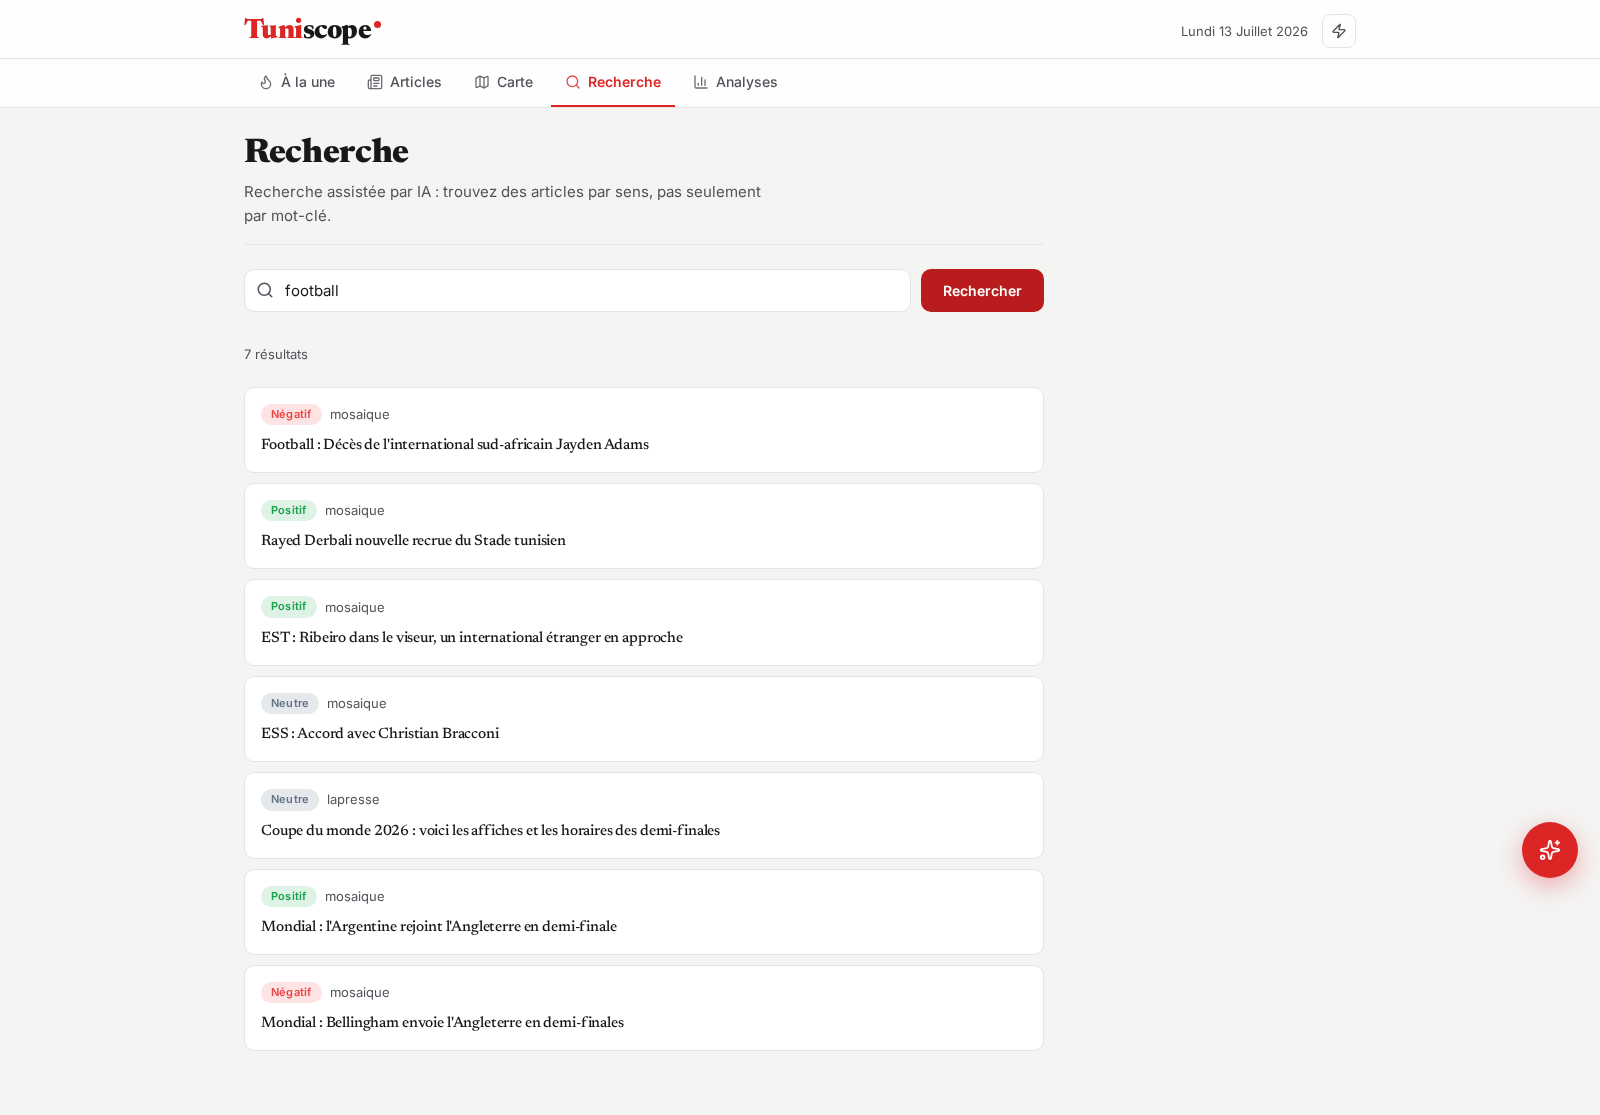
\includegraphics[width=0.9\columnwidth]{img/screen-search.png}
\caption{The AI-assisted semantic search results view (\texttt{Search.jsx}): each result carries its sentiment badge, source, and topic label alongside the query match.}
\label{fig:screen-search}
\end{figure}

\section{Ask-the-news chat assistant}
\label{sec:chat-assistant}
\begin{sloppypar}
\texttt{POST /genai/chat} (\texttt{chat}, \texttt{api/\allowbreak routes/\allowbreak genai.py}) accepts a single field, \texttt{q}, and implements a small retrieval-augmented-generation loop. Retrieval follows the same cached-embedding check as search: if \texttt{embeddings\_available()}, the question is embedded (with the \texttt{"query: "} prefix described in Chapter 4) and the five nearest articles are fetched by \texttt{ORDER BY embedding <=> \%s::vector LIMIT 5}; otherwise, the same French full-text machinery used elsewhere ranks by \texttt{ts\_rank} and falls back to \texttt{COALESCE(published\_at, scraped\_at)} recency, again \texttt{LIMIT 5}. The comment in the code is explicit about why this path always returns five rows rather than nothing on a weak match: chat needs \emph{some} grounding context to answer at all, unlike search, which must never show the reader an article it cannot justify. The five retrieved rows -- \texttt{id, title, url, content} -- are then folded into one numbered context block (Listing~6.2): each article becomes \texttt{"[n] title\textbackslash ncontent[:800]"}, joined by blank lines, giving the model up to 800 characters of body text per source.
\end{sloppypar}

\begin{verbatim}
context = "\n\n".join(
    f"[{i+1}] {r[1]}\n{(r[3] or '')[:800]}"
    for i, r in enumerate(rows)
)
\end{verbatim}
\begin{center}
\textit{Listing~6.2: building the numbered RAG context (\texttt{chat}, \texttt{api/routes/genai.py}) -- five retrieved articles become five bracketed, citable sources.}
\end{center}

\begin{sloppypar}
That context, together with the question, is sent to \texttt{complete} with a system prompt instructing the model to answer strictly from the supplied articles, cite their source numbers, and say so explicitly if the answer is not in them; the model is resolved through \texttt{model\_for("chat", DEFAULT\_MODEL)} -- \texttt{llama-3.3-70b-\allowbreak versatile} by default -- and capped at \texttt{max\_tokens=512}. The endpoint returns \texttt{\{"answer": ..., "sources": [\{"id", "title", "url"\}, \ldots]\}}, with \texttt{sources} always listing all five retrieved articles regardless of which bracket numbers the generated answer actually cites, leaving it to the frontend to present them as the full evidence set rather than a filtered citation list. \texttt{ChatWidget.jsx} renders this as a floating assistant: a round action button toggles a docked panel offering three canned French suggestions on an empty conversation (\emph{``Que se passe-t-il en Tunisie cette semaine ?''} among them), posts each question to \texttt{/genai/chat}, appends the returned answer as an assistant bubble with its sources rendered as a bulleted list of clickable external links, and -- on a failed request -- appends a generic French error bubble instead of the answer, catching the failure entirely on the client. Figure~\ref{fig:screen-chat} shows the assistant open with an answered question and its cited sources.
\end{sloppypar}

\begin{figure}[H]
\centering

\includegraphics[width=0.9\columnwidth]{img/screen-chat.png}
\caption{The ``ask the news'' chat assistant (\texttt{ChatWidget.jsx}): a RAG answer over five retrieved articles, with clickable source citations.}
\label{fig:screen-chat}
\end{figure}

\section{Cost and reliability considerations}
\label{sec:genai-cost}
\begin{sloppypar}
Every design choice in this chapter traces back to running LLM features on a free tier without a card on file. The fast/strong model split (Section~\ref{sec:llm-provider}) is the main lever: \texttt{FAST\_MODEL} absorbs the highest-volume traffic -- one \texttt{classify\_theme} call per ingested article, one \texttt{label\_topics} call per BERTopic cluster, one summary call per distinct article ever opened -- while \texttt{DEFAULT\_MODEL} is reserved for the lower-volume, higher-stakes calls: one per chat question, and, since the precision fix, one per AI-search request that reaches the ranking step. Summaries add a second lever on top, a persistent cache in \texttt{articles.summary}: the same article is never summarized twice, regardless of how many readers open it, which chat has no equivalent for since every question is, by construction, distinct. Because \texttt{LLM\_BASE\_URL}/\texttt{LLM\_MODEL} are the only inputs \texttt{etl/llm.py} needs, the whole system can also move off Groq entirely -- to Gemini for better French and a longer context window, or to an OpenRouter \texttt{:free} model for a different rate-limit profile -- without a code change, exactly as the README documents.
\end{sloppypar}

\begin{sloppypar}
Reliability is handled asymmetrically across the codebase, and not by accident. \texttt{\_client()} configures no explicit request timeout or retry policy, so every call to \texttt{complete} inherits whichever defaults the underlying \texttt{openai} Python SDK (and the \texttt{httpx} client it wraps) ships with. Chapter 5's three enrichment functions -- \texttt{classify\_theme}, \texttt{label\_topics}, \texttt{tag\_region\_llm} -- and this chapter's \texttt{\_ai\_rank} all wrap their own \texttt{complete} call in a \texttt{try/except} that degrades to a hard-coded default (``Société,'' \texttt{f"Topic \{tid\}"}, an unmatched region, an empty ranking list) rather than raising, so a provider outage during a batch pipeline run or a search request lowers output quality without aborting anything. The two live, user-triggered endpoints in \texttt{api/\allowbreak routes/\allowbreak genai.py}, \texttt{summary} and \texttt{chat}, do not follow that pattern: neither wraps its \texttt{complete} call in a \texttt{try/except}, so a provider error at request time propagates as an unhandled exception and FastAPI turns it into a 500 response. Both frontend call sites already assume this can happen and handle it locally instead of relying on the backend to degrade gracefully: \texttt{ArticleModal.jsx}'s \texttt{ArticleSummary} catches the failed request and simply renders no summary box at all, and \texttt{ChatWidget.jsx}'s \texttt{ask} catches it and appends a generic French error bubble to the conversation rather than leaving the user staring at a stalled spinner.
\end{sloppypar}

\section{Conclusion}
\begin{sloppypar}
A single, roughly fifty-line module, \texttt{etl/llm.py}, underlies every LLM-backed feature this report has described across two chapters: theme classification and topic labelling at ingestion time (Chapter 5), and article summaries, AI-assisted search ranking, and the ask-the-news chat assistant covered here -- all swappable to a different provider through three environment variables, and individually re-modelled through three more. Two real fixes drawn directly from the project's commit history illustrate that this is a system that was actually run and iterated on rather than designed once and left alone: a scraper-plus-prompt fix for articles too short for the model to summarize, and a stronger-model-plus-stricter-fallback fix for search results that drifted into unrelated recent news whenever the ranking step failed. The next chapter turns from these individual features to how the whole pipeline that feeds them is orchestrated and observed in production: Prefect flows and MLflow experiment tracking.
\end{sloppypar}
